Evaluation of ESN performance on the NARMA system is a thoroughly explored area
in the field of RC \cite{verstraeten_experimental_2007, rodan_minimum_2011,
jaeger_adaptive_nodate}. Similar performance to previous work has been achieved
(Fig. \ref{visualization}, \ref{performance}) as a baseline to lend credibility
to further approaches in this paper.

\begin{figure}[H]
  \centering
  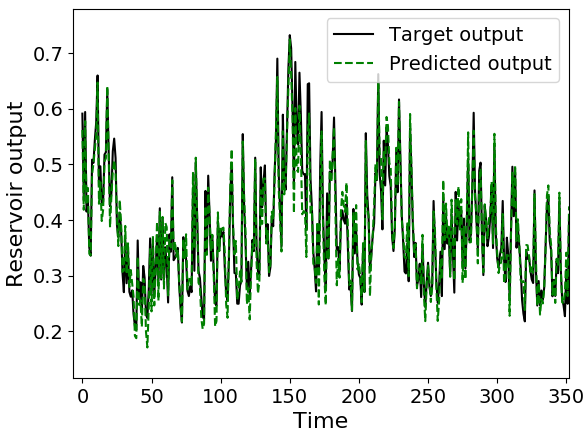
\includegraphics[width=2.5in]{img/narma_visualization.png}
  \caption{
    Visualization of reservoir output when fed the NARMA10 task. Input is an
i.i.d. stream generated uniformly in the interval [0, 0.5].
  }
  \label{visualization}
\end{figure}

\begin{figure}[H]
  \centering
  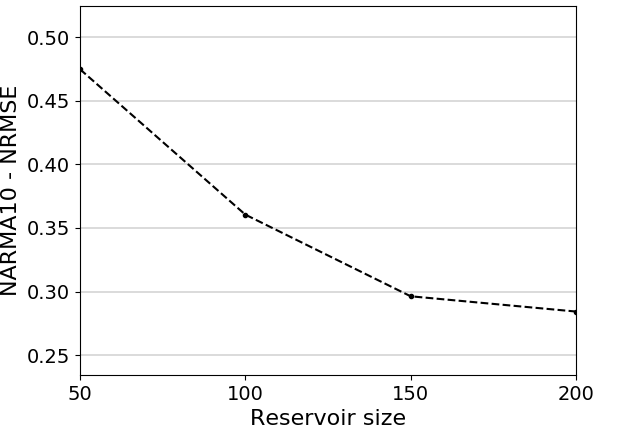
\includegraphics[width=2.5in]{img/general_performance.png}
  \caption{
    Reservoir size versus ESN performance for the NARMA10 task. The NRMSE is
averaged over 10 simulation runs.
  }
  \label{performance}
\end{figure}

All further reservoirs were constructed with the parameters from this baseline:
$\mathbf{W}^{res}$ and $\mathbf{W}^{in}$ were both generated as random matrices
with i.i.d. entries in the interval [-0.5, 0.5]. Both matrices are fully
connected, and the reservoir weight matrix was rescaled to have a spectral
radius of 0.9.

% (TODO): w_res density was also set to 0.2.

% (TODO): Sizes we use for NARMA training and testing.

% (TODO): The code base is available at <link>.

% (TODO): All experiments are conducted with 10 reservoirs per point.

\subsection{Noise}

Physical, real world systems are affected by noise. By extension, designers of
reservoirs that use material substrates must be aware of the effects the noise
that is present may have on computational power.

Additive white Gaussian noise (AWGN) is a common noise model that mimics the
noise patterns of many random processes in nature. The noise is additive,
meaning the AWGN output is the sum of the input $u_{i}$ and the noise values
$v_{i}$. $v_{i}$ is i.i.d and drawn from a Gaussian distribution with zero-mean,
and a variance $\sigma^{2}$.

Here we model noise by extending the ESN model to take the sum of two individual
inputs, $u$ and $v$, which represent the signal and the noise. The goal of the
reservoir remains a computation on the signal $u$, a task now hindered by the
unwanted noise.

We first vary the signal to noise ratio of noise when running the test dataset
without imposing any noise during training. In this case we see the inherent
robustness of the reservoirs to undesired noise that is previously unseen. The
results are shown in Fig. \ref{input_noise_snr}, illustrating a performance
degradation when the ratio of signal power to noise power drops below 20, which
corresponds to AWGN with standard deviation $\sigma \approx 0.0144$. Similar
performance degradation was seen in \cite{dambre_information_2012}, where the
same SNR measure was used to evaluate the reconstruction capacity from the state
of a dynamical system.

A comparison can be drawn to commonly recommended SNRs in the IEEE 802.11
standard for Wi-Fi communications, ranging from 15db to 25dB. Below this
threshold, wireless communication will quickly become unusable.



% (TODO): Find some more info about noise from Verstraeten paper^. To compare with
% this paragraph.

% (TODO): Key point: as long as we train with noise, we become more
% robust. However, this is only in the case where the performance _really_ breaks
% down.

% (TODO): Write a little about AWGN.

\begin{figure}[H]
  \centering
  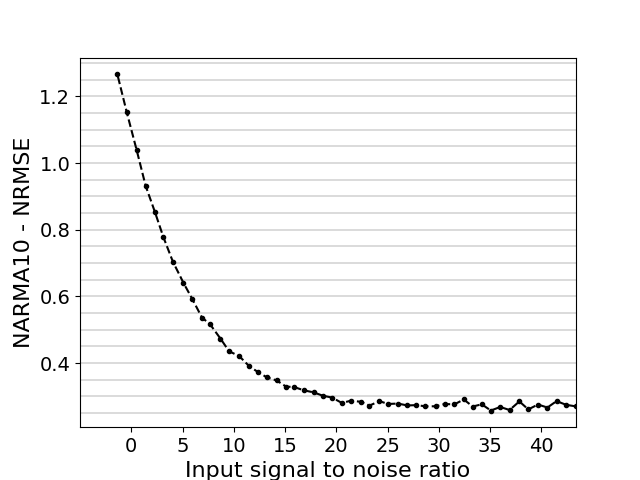
\includegraphics[width=2.5in]{img/input_noise_snr.png}
  \caption{
    Noise causing a decrease in performance of a reservoir with 200 hidden nodes
on the NARMA10 task. Input signal to noise ratio is measured in dB, and is
calculated as $SNR = 10\log_{10}(\frac{var(u)}{var(v)})$, the measure also used
in \cite{dambre_information_2012}.
  }
  \label{input_noise_snr}
\end{figure}

Some text.

\begin{figure}[H]
  \centering
  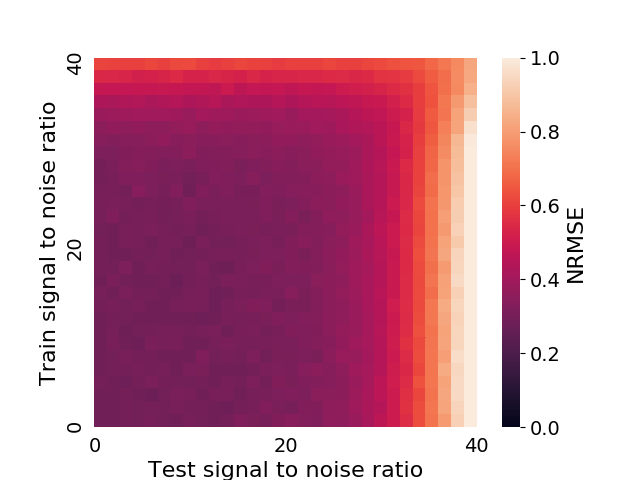
\includegraphics[width=2.5in]{img/input_noise_heatmap.png}
  \caption{
    Input noise signal to noise ratio for test/train.
  }
  \label{input_noise_heatmap}
\end{figure}

More text.

\subsection{Measurement equipment accuracy}

When conducting experiments using physical reservoirs, one will inevitably have
to interact with substrates from software. Whether it be transforming digital
representations of reservoir perturbations to analog signals that cause the
excitation, or the reverse mapping of the analog state of the reservoir into a
digital representation, the accuracy of equipment used for such conversions is
of crucial importance.

Sensor anomalies, noise, and amplification gain may all impact performance, but
as found in the previous subsection, reservoirs prove to be quite robust to the
presence of such noise patterns. Here we thus focus our investigation on the
quantization done in ADC systems.

% (TODO): There are common ADC errors: gain error, linearity error, missing code
% errors, offset errors.

\begin{figure}[H]
  \centering
  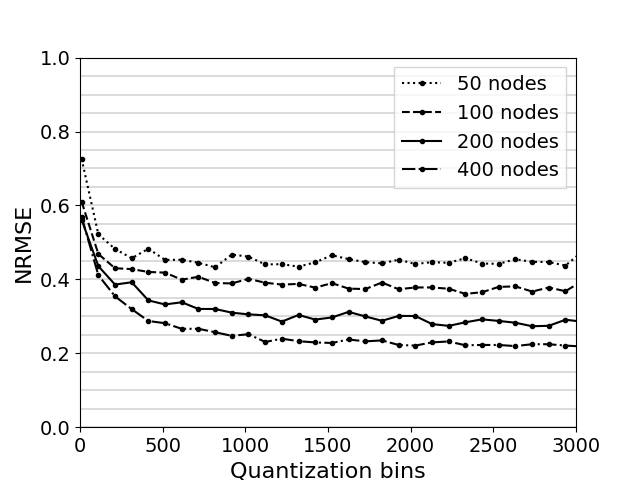
\includegraphics[width=2.5in]{img/adc_quantization.png}
  \caption{
    Performance effect of ADC quantization on four reservoirs of different
sizes. $\tanh$ is used as activation function for the experiment, dividing its
range of (1-, 1) into $n$ discrete output bins.
  }
  \label{adc_quantization}
\end{figure}

To emulate the behavior of an ADC, we extend our ESN model to allow for
quantization of reservoir output before it is passed to the readout layer. This
quantization effectively divides the range of the nonlinear activation function
of each hidden node into a discrete set of fixed output bins.

Fig. \ref{adc_quantization} shows how quantization affects reservoir
performance. We plot the error of four different reservoir sizes: 50, 100, 200
and 400 hidden nodes.

We see a performance degradation from 3000 to 1000 discernible states, something
of which is more pressing for the bigger reservoirs. As discrete output states
move beneath 1000, the performance quickly deteriorates. However, even with just
10 discrete outputs, reservoirs are still able to replicate the input sequence
to some degree. Furthermore, reservoirs with 400 hidden nodes and just 100
discrete output bins consistently provide the same performance as that of a
reservoir with 50 hidden nodes and no output quantization.

A 12-bit ADC has $2^{12}$, or 4096 output codes, which in accordance with our
experiments would impose no noticeable increase in the prediction error. 16-bit
ADCs, outputting $2^{16}$, or 65536 discrete states, would influence our ESN
simulations even less. In \cite{soriano_delay-based_2015}, a major factor
limiting performance of a delay-based RC implementation was quantization noise,
where low error rates were achieved with 8 bits or more in the ADC. This result
is also seen in our ESN implementation, where NRMSE starts leveling out around 8
bits of accuracy, or 256 discrete states.

These results demonstrate that the reservoir methodology provides an inherent
resilience to output quantization. When designing physical RC systems, this may
be applied in preliminary analysis of the output resolution and representation,
whether it be voltage in electrode arrays or the magnetic polarization of
permalloy nanomagnets.

% (TODO): I don't really like the conclusion here -- could I conclude with
% something more _concrete_, almost like tricks of the trade?

% (TODO): Would higher order NARMAs show different degradations, as they require
% more memory and computation?

\subsection{Partially visible state}

\begin{figure}[H]
  \centering
  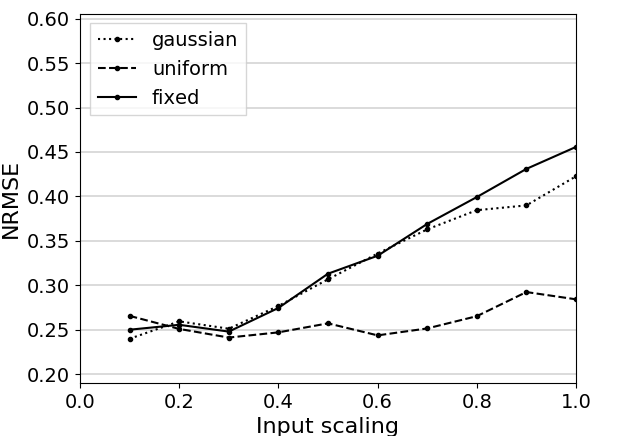
\includegraphics[width=2.5in]{img/input_scaling_distrib.png}
  \caption{
    Effect of input scaling on three input weight distributions.
  }
  \label{input_scaling_distrib}
\end{figure}

\begin{figure*}[htbp]
  \centering
  \begin{subfigure}{.3\textwidth}
    \centering
    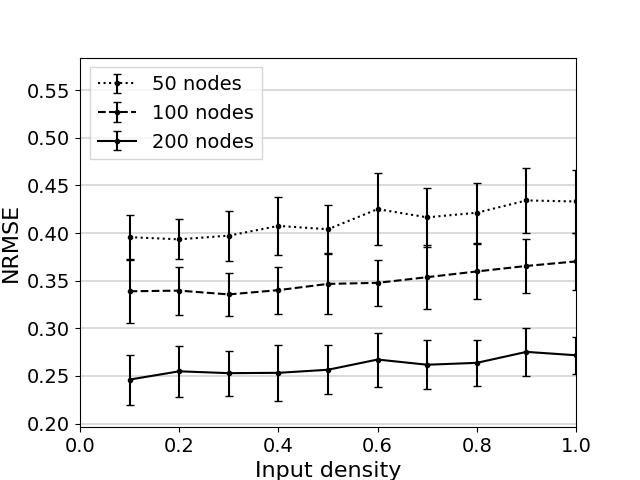
\includegraphics[width=\linewidth]{img/input_density_all.png}
  \end{subfigure}
  \begin{subfigure}{.3\textwidth}
    \centering
    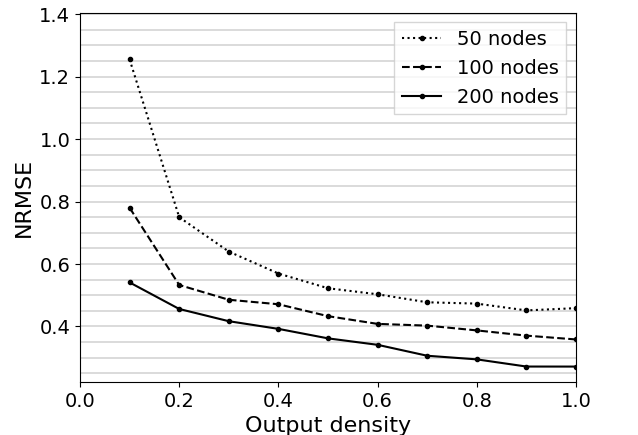
\includegraphics[width=\linewidth]{img/output_density_all.png}
  \end{subfigure}
  \begin{subfigure}{.3\textwidth}
    \centering
    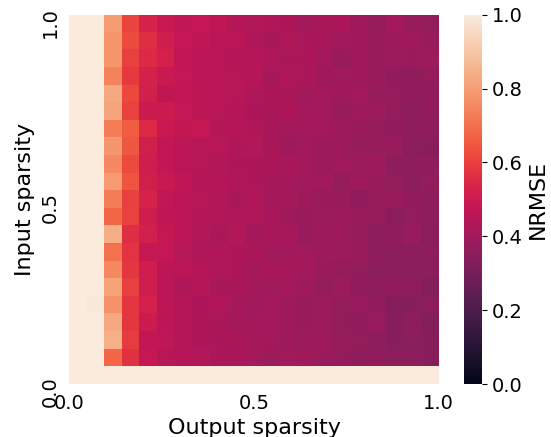
\includegraphics[width=\linewidth]{img/partial_visibility.png}
  \end{subfigure}
  \caption{
    These figures show the influence of reservoirs that are only partially
visible on the performance for the NARMA10 task. Experiments for the rightmost
plot were conducted using a reservoir size of 200 hidden nodes. The density is a
measurement for the fraction of elements in the input and output matrices
containing non-zero elements.
  }
  \label{partial_visibility}
\end{figure*}

% (TODO): Tie this together with topology, if it has a feed-forward-like structure
% or similar.

% (TODO): Elaborate on global input, works the most. In fact all the way down to
% 0.18 NRMSE, which is excellent.

\subsection{Topology}

\begin{figure}[H]
  \centering
  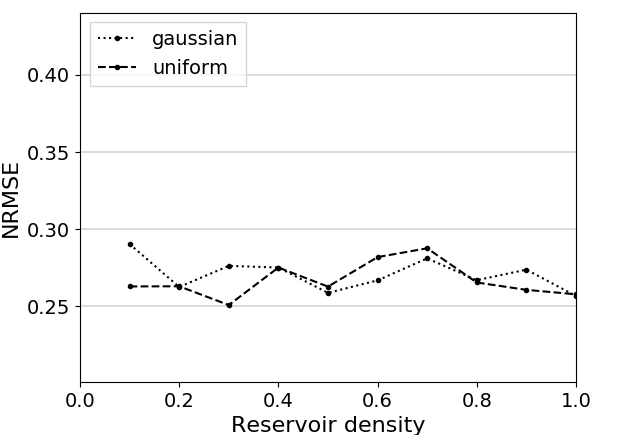
\includegraphics[width=2.5in]{img/reservoir_density_distrib.png}
  \caption{
    Reservoir density versus for two weight distributions. Fixed weight will not
work for internal nodes, unless special topology is employed, e.g. ring
(elaborate). This shows that sparse internal weight matrices work fine.
  }
  \label{reservoir_density_distrib}
\end{figure}

% (TODO): Is w_density also interesting for physical reservoirs?

%%% Local Variables:
%%% mode: latex
%%% TeX-master: "../main"
%%% End:
